\documentclass{article}

\usepackage{graphicx}
\usepackage{tikz}
\usepackage{tikzsymbols}
\usetikzlibrary{calc,patterns,shapes.geometric}
\pagestyle{empty}
\usepackage[margin=0pt]{geometry}
\geometry{papersize={14in,12in}}

\def\centerarc[#1](#2)(#3:#4:#5){\draw[#1] ($(#2)+({#5*cos(#3)},{#5*sin(#3)})$) arc (#3:#4:#5);}

\begin{document}
	\begin{figure}
		\centering
		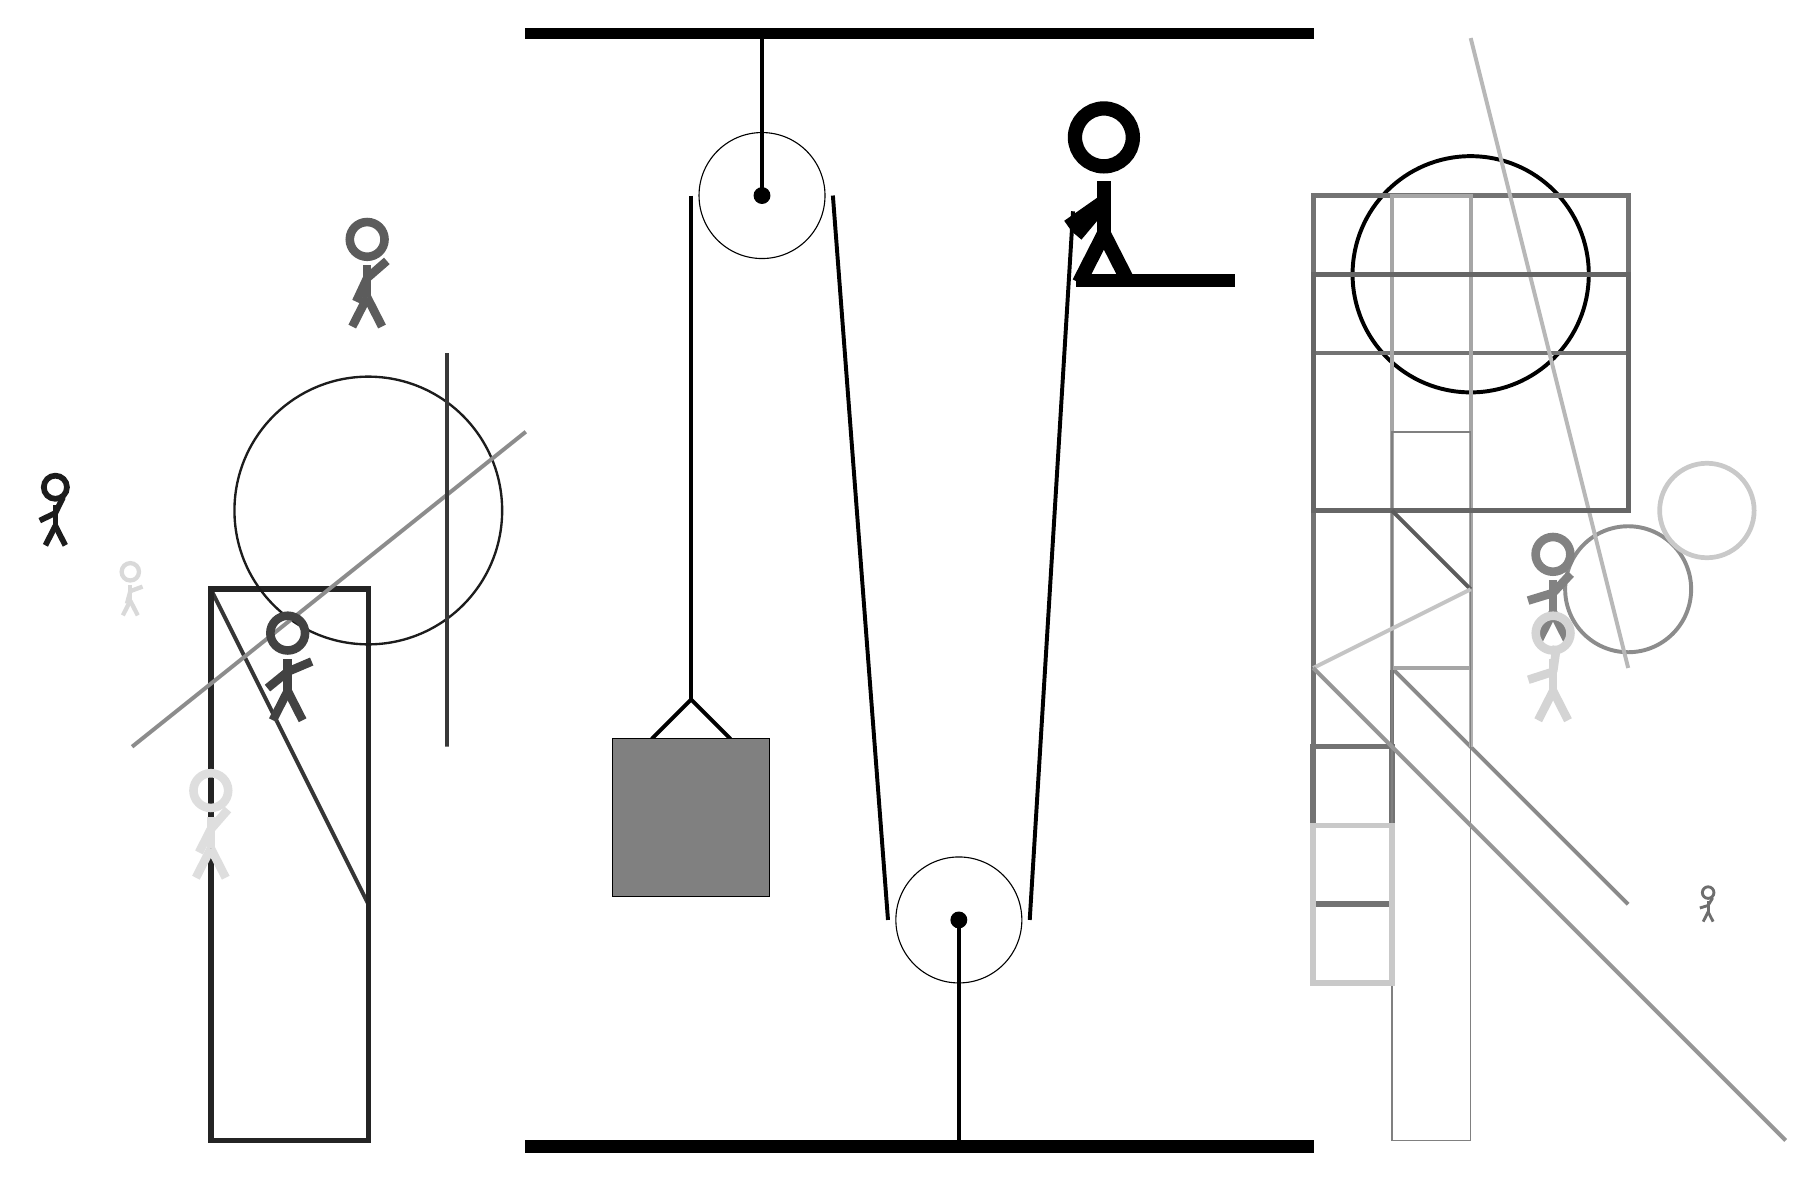
\begin{tikzpicture}
			%%%%% START %%%%%
			
			\draw[fill=black] (-2, 14) rectangle (8, 14.125);
			
			\draw (3.5, 2.8) circle (0.8);
			\draw[fill=black] (3.5, 2.8) circle (0.1);
			\draw[line width=0.5mm] (3.5, 2.8) -- (3.5, 0);
			
			\draw (1, 12) circle (0.8);
			\draw[fill=black] (1, 12) circle (0.1);
			\draw[line width=0.5mm] (1, 14) -- (1, 12);
			
			\draw[line width=0.5mm](-0.4, 5.1) --  (0.1, 5.6) -- (0.6, 5.1);
			\draw[fill=black!50] (-0.9, 5.1) rectangle (1.1, 3.1);
			
			\draw[line width=0.5mm](0.1, 12) -- (0.1, 5.6);
			\centerarc[line width=0.5mm](1, 12)(180:0:0.9)
			\draw[line width=0.5mm](1.9, 12) -- (2.6, 2.8);
			\centerarc[line width=0.5mm](3.5, 2.8)(180:360:0.9)
			\draw[line width=0.5mm](4.4, 2.8) -- (4.95, 11.8);
			
			\draw [line width=0.5mm, color=black!45](12, 7) circle (0.8);
			
			\node[line width=0.6mm, color=black!49] at (11, 7) {\Strichmaxerl[6][17][47]};
			\draw [line width=0.5mm, color=black!100](10, 11) circle (1.5);
			\draw[line width=0.5mm, color=black!79](-6, 7) -- (-4, 3);
			
			\draw[line width=0.7mm, color=black!86] (-4, 7) rectangle (-6, 0);
			\draw[line width=0.6mm, color=black!55] (8, 10) rectangle (12, 12);
			\draw[line width=0.5mm, color=black!46](12, 3) -- (9, 6);
			\draw[line width=0.6mm, color=black!55] (9, 12) rectangle (8, 3);
			\draw [line width=0.3mm, color=black!89](-4, 8) circle (1.7);
			\draw[line width=0.5mm, color=black!45](-7, 5) -- (-2, 9);
			\draw[line width=0.5mm, color=black!31](10, 5) -- (10, 12);
			\node[line width=0.3mm, color=black!17] at (11, 6) {\Strichmaxerl[6][18][82]};
			\node[line width=0.5mm, color=black!57] at (13, 3) {\Strichmaxerl[2][17][59]};
			
			\draw[line width=0.5mm, color=black!35] (10, 12) rectangle (9, 6);
			\node[line width=0.6mm, color=black!74] at (-5, 6) {\Strichmaxerl[6][39][23]};
			\draw[line width=0.7mm, color=black!55] (8, 5) rectangle (9, 3);
			\draw[line width=0.5mm, color=black!28](12, 6) -- (10, 14);
			\node[line width=0.4mm, color=black!15] at (-7, 7) {\Strichmaxerl[3][75][20]};
			\draw[line width=0.2mm, color=black!50] (10, 0) rectangle (9, 9);
			\draw[line width=0.6mm, color=black!60] (8, 8) rectangle (12, 11);
			\draw[line width=0.5mm, color=black!78] (-3, 10) rectangle (-3, 5);
			
			\draw[line width=0.5mm, color=black!64](9, 8) -- (10, 7);
			\node[line width=0.4mm, color=black!13] at (-6, 4) {\Strichmaxerl[6][63][49]};
			\node[line width=0.2mm, color=black!64] at (-4, 11) {\Strichmaxerl[6][65][41]};
			\draw[line width=0.7mm, color=black!21] (9, 4) rectangle (8, 2);
			
			\draw[line width=0.5mm, color=black!23](10, 7) -- (8, 6);
			\draw [line width=0.6mm, color=black!21](13, 8) circle (0.6);
			\node[line width=0.7mm, color=black!89] at (-8, 8) {\Strichmaxerl[4][26][64]};
			
			\draw[line width=0.5mm, color=black!41](8, 6) -- (14, 0);
			
			\node at (5.3, 12) {\Strichmaxerl[10][35][-130]};
			\draw[fill=black] (5, 11) rectangle (7, 10.85);
			
			\draw[fill=black] (-2, 0) rectangle (8, -0.15);
			
			%%%%% END %%%%%
		\end{tikzpicture}
	\end{figure}	
\end{document}